% Title of the article

\documentclass[12 pt]{article}
%\documentclass[12 pt, draft]{article} % hizalama problemlerini gösterir ve bağlantıları etkisiz hâle getirir

%%%%%%% PAKETLER %%%%%%%

% elzem paketler

\usepackage[utf8]{inputenc}
\usepackage[margin = 2.54 cm]{geometry} % Flexible and complete interface to document dimensions
\usepackage{setspace} % Set space between lines
	\doublespacing
\usepackage{authblk} % Support for footnote style author/affiliation (yazarların kurum bilgilerinin yazım şekliyle ilgili değişiklikler yapabilmek ve bu kısmın satır arası boşluğunu azaltmak için)
	\renewcommand\Affilfont{\itshape\normalsize} % kurum bilgisi yazı karakterini değiştirmek için
\usepackage{mathtools}
\usepackage{natbib} % Flexible bibliography support
	\bibliographystyle{plainnat}
	\bibpunct{(}{)}{;}{a}{,}{,}
	% bk. https://www.ctan.org/pkg/natbib sayfasında Reference Sheet
\usepackage{doi}

% sıklıkla lazım olan paketler

\usepackage{tabularx, caption}
	\renewcommand{\tabularxcolumn}[1]{>{\normalsize}m{#1}} % hücre içeriklerini dikey ortalamak için
	\newcolumntype{Y}{>{\normalsize\centering\arraybackslash}X} % yatay ortalanmış sütun biçimi
\usepackage{graphicx} % resim ekleyebilmek için
	\graphicspath{{./auxiliary/}} % resimler -varsa- auxiliary klasörü içinde
\usepackage{tikz} % çizim yapabilmek için
\usepackage{algpseudocodex} % sözde kod yazabilmek için

\usepackage{ulem} % Package for underlining (revizyonda silinen kısımları göstermek için)

\usepackage{lipsum} % işbu şablonda kullanmak üzere

%%%%%%% KOMUTLAR %%%%%%%

\newcommand{\desktop}{PC with Intel(R) Core(TM) i7-4790 CPU (3.60 GHz) and 8 GB RAM} % Acer ofis (masaüstü) bilgisayarı

%%%%%%% BAŞLIK VE YAZAR BİLGİSİ %%%%%%%

\title{
Title of the article%
\bigskip
}

\author{
Murat Güngör \\
Industrial Engineering Department, Istanbul Medeniyet University \\
34700, Istanbul, Turkey \\
\textup{\texttt{murat.gungor@medeniyet.edu.tr}} \\
\textup{\texttt{\href{https://orcid.org/0000-0002-7202-6619}{https://orcid.org/0000-0002-7202-6619}}}
}

%\author{} % çift taraflı kör hakemlikte yazar bilgisini gizlemek için
  
\date{} % 12 Mart 2025

%%%%%%% MAKALE (İNGİLİZCE) %%%%%%%

\begin{document}

\maketitle

\thispagestyle{empty} % ilk sayfayı numaralandırmamak için

%\newpage % gerekirse başlık sayfası (title page) için

\begin{abstract}
\lipsum[1]
\end{abstract}

\begin{small}
\begin{center}
\textbf{Keywords} \\[4pt]
first keyword; second keyword; third keyword; fourth keyword
\end{center}
\end{small}

\section{Introduction}
\label{sec:intro}

\lipsum[2-3]

\section{Second section}
\label{sec:second}

\subsection{First subsection}
\label{subsec:first}

\lipsum[4]

\subsection{Second subsection}
\label{subsec:second}

\lipsum[5]

\section*{Tables and figures}

\lipsum[6]

\begingroup
\renewcommand{\arraystretch}{1.25}
\begin{table}[h]
\centering
\caption{Caption of the table.}
\label{tab:notation}
\begin{tabular}{c l}
\hline
Symbol & Explanation \\
\hline
$a$ & first symbol \\
$b$ & second symbol \\
$c$ & third symbol \\
\hline
\end{tabular}
\end{table}
\endgroup
% burada boşluk olup olmaması bir şey değiştirmiyor
\lipsum[7]

\bigskip % metni resimden biraz uzaklaştırmak için

\begin{figure}[h]
\centering
\includegraphics[scale = 0.15]{logo}
\caption{Caption of the figure.}
\label{fig:logo}
\end{figure}
% burada boşluk olup olmaması bir şey değiştirmiyor
\lipsum[8]

\bigskip % metni resimden biraz uzaklaştırmak için

\begingroup
\begin{figure}[h]
\centering
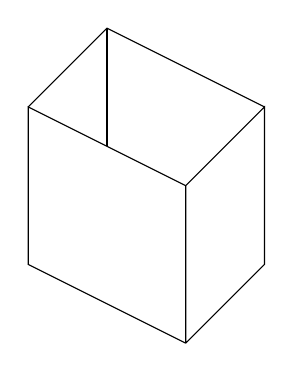
\begin{tikzpicture}
\begin{footnotesize}
\draw (0, 0) -- (1, 1) -- (1, 3) -- (0, 2) -- (0, 0);
\draw (0, 0) -- (-2, 1) -- (-2, 3) -- (0, 2);
\draw (-2, 3) -- (-1, 4) -- (1, 3);
\draw (-1, 4) -- (-1, 2.5);
\end{footnotesize}
\end{tikzpicture}
\caption{Caption of the drawing.}
\label{fig:drawing}
\end{figure}
\endgroup

\lipsum[9]

\bigskip % metni resimden biraz uzaklaştırmak için

\begin{figure}[h]
\centering
\fbox
{
\begin{minipage}{0.33\textwidth}
\medskip
\begin{algorithmic}
\State $\varepsilon \gets 1$
\While {$1 + \varepsilon > 1$}
	\State $\varepsilon \gets \varepsilon/2$
\EndWhile
\State \Output {$\varepsilon$}
\end{algorithmic}
\medskip
\end{minipage}
}
\caption{Caption of the pseudocode.}
\label{fig:pseudocode}
\end{figure}

\lipsum[10]

\section*{Citations}

Section~\ref{sec:intro}...\\
Subsection~\ref{subsec:first}...\\
Table~\ref{tab:notation}...\\
Figure~\ref{fig:logo}...\\
\cite{VanLoon2015}...\\
(\citealp{VanLoon2015})...\\
(\citealp{VanLoon2015, Hyndman2021})...\\

\section*{Revision}

\sout{text to be deleted} \textcolor{red}{text to be added}

\section*{Statements and declarations}

\subsection*{Acknowledgments}

\lipsum[11][1-3]

\subsection*{Competing interests}

The author has no relevant financial or non-financial interests to disclose.

\subsection*{Availability of data and materials}

\lipsum[11][4-6]

\subsection*{Funding}

This research did not receive any specific grant from funding agencies in the public, commercial, or not-for-profit sectors.

%\bibliography{library} % library dosyası işbu TeX dosyası ile aynı klasörde ise
\bibliography{auxiliary/library} % library dosyası auxiliary klasörü içinde ise

\end{document}